% Created by tikzDevice version 0.7.0 on 2015-03-24 13:59:03
% !TEX encoding = UTF-8 Unicode
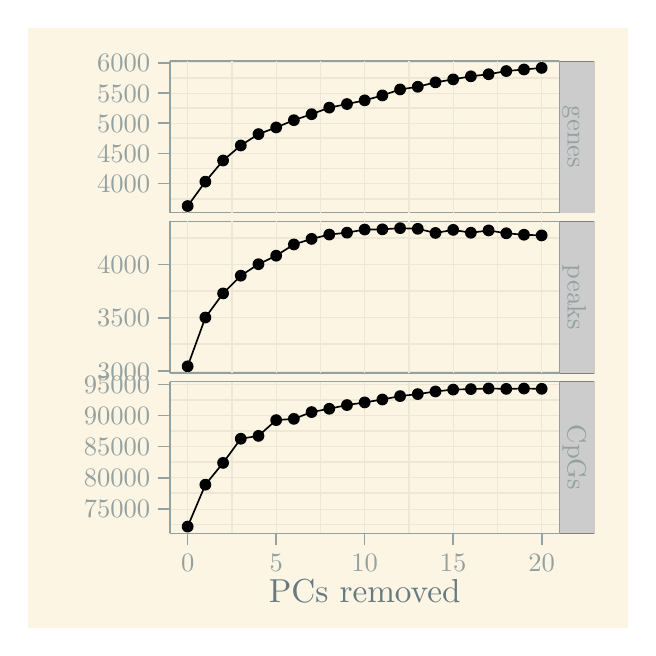
\begin{tikzpicture}[x=1pt,y=1pt]
\definecolor[named]{fillColor}{rgb}{0.99,0.96,0.89}
\path[use as bounding box,fill=fillColor] (0,0) rectangle (216.81,216.81);
\begin{scope}
\path[clip] (  0.00,  0.00) rectangle (216.81,216.81);

\path[fill=fillColor] (  0.00,  0.00) rectangle (216.81,216.81);
\end{scope}
\begin{scope}
\path[clip] ( 51.42,149.86) rectangle (192.13,204.77);
\definecolor[named]{drawColor}{rgb}{0.58,0.63,0.63}
\definecolor[named]{fillColor}{rgb}{0.99,0.96,0.89}

\path[draw=drawColor,line width= 0.6pt,line join=round,line cap=round,fill=fillColor] ( 51.42,149.86) rectangle (192.13,204.77);
\definecolor[named]{drawColor}{rgb}{0.93,0.91,0.84}

\path[draw=drawColor,line width= 0.6pt,line join=round] ( 51.42,155.00) --
	(192.13,155.00);

\path[draw=drawColor,line width= 0.6pt,line join=round] ( 51.42,165.92) --
	(192.13,165.92);

\path[draw=drawColor,line width= 0.6pt,line join=round] ( 51.42,176.84) --
	(192.13,176.84);

\path[draw=drawColor,line width= 0.6pt,line join=round] ( 51.42,187.77) --
	(192.13,187.77);

\path[draw=drawColor,line width= 0.6pt,line join=round] ( 51.42,198.69) --
	(192.13,198.69);

\path[draw=drawColor,line width= 0.6pt,line join=round] ( 73.80,149.86) --
	( 73.80,204.77);

\path[draw=drawColor,line width= 0.6pt,line join=round] (105.78,149.86) --
	(105.78,204.77);

\path[draw=drawColor,line width= 0.6pt,line join=round] (137.76,149.86) --
	(137.76,204.77);

\path[draw=drawColor,line width= 0.6pt,line join=round] (169.74,149.86) --
	(169.74,204.77);

\path[draw=drawColor,line width= 0.2pt,line join=round] ( 51.42,160.46) --
	(192.13,160.46);

\path[draw=drawColor,line width= 0.2pt,line join=round] ( 51.42,171.38) --
	(192.13,171.38);

\path[draw=drawColor,line width= 0.2pt,line join=round] ( 51.42,182.30) --
	(192.13,182.30);

\path[draw=drawColor,line width= 0.2pt,line join=round] ( 51.42,193.23) --
	(192.13,193.23);

\path[draw=drawColor,line width= 0.2pt,line join=round] ( 51.42,204.15) --
	(192.13,204.15);

\path[draw=drawColor,line width= 0.2pt,line join=round] ( 57.81,149.86) --
	( 57.81,204.77);

\path[draw=drawColor,line width= 0.2pt,line join=round] ( 89.79,149.86) --
	( 89.79,204.77);

\path[draw=drawColor,line width= 0.2pt,line join=round] (121.77,149.86) --
	(121.77,204.77);

\path[draw=drawColor,line width= 0.2pt,line join=round] (153.75,149.86) --
	(153.75,204.77);

\path[draw=drawColor,line width= 0.2pt,line join=round] (185.73,149.86) --
	(185.73,204.77);
\definecolor[named]{fillColor}{rgb}{0.00,0.00,0.00}

\path[fill=fillColor] ( 57.81,152.36) circle (  2.13);

\path[fill=fillColor] ( 64.21,161.16) circle (  2.13);

\path[fill=fillColor] ( 70.61,168.81) circle (  2.13);

\path[fill=fillColor] ( 77.00,174.24) circle (  2.13);

\path[fill=fillColor] ( 83.40,178.35) circle (  2.13);

\path[fill=fillColor] ( 89.79,180.75) circle (  2.13);

\path[fill=fillColor] ( 96.19,183.38) circle (  2.13);

\path[fill=fillColor] (102.59,185.54) circle (  2.13);

\path[fill=fillColor] (108.98,187.92) circle (  2.13);

\path[fill=fillColor] (115.38,189.21) circle (  2.13);

\path[fill=fillColor] (121.77,190.54) circle (  2.13);

\path[fill=fillColor] (128.17,192.33) circle (  2.13);

\path[fill=fillColor] (134.57,194.49) circle (  2.13);

\path[fill=fillColor] (140.96,195.45) circle (  2.13);

\path[fill=fillColor] (147.36,197.05) circle (  2.13);

\path[fill=fillColor] (153.75,198.12) circle (  2.13);

\path[fill=fillColor] (160.15,199.23) circle (  2.13);

\path[fill=fillColor] (166.55,199.98) circle (  2.13);

\path[fill=fillColor] (172.94,201.13) circle (  2.13);

\path[fill=fillColor] (179.34,201.70) circle (  2.13);

\path[fill=fillColor] (185.73,202.27) circle (  2.13);
\definecolor[named]{drawColor}{rgb}{0.00,0.00,0.00}

\path[draw=drawColor,line width= 0.6pt,line join=round] ( 57.81,152.36) --
	( 64.21,161.16) --
	( 70.61,168.81) --
	( 77.00,174.24) --
	( 83.40,178.35) --
	( 89.79,180.75) --
	( 96.19,183.38) --
	(102.59,185.54) --
	(108.98,187.92) --
	(115.38,189.21) --
	(121.77,190.54) --
	(128.17,192.33) --
	(134.57,194.49) --
	(140.96,195.45) --
	(147.36,197.05) --
	(153.75,198.12) --
	(160.15,199.23) --
	(166.55,199.98) --
	(172.94,201.13) --
	(179.34,201.70) --
	(185.73,202.27);
\end{scope}
\begin{scope}
\path[clip] ( 51.42, 91.95) rectangle (192.13,146.85);
\definecolor[named]{drawColor}{rgb}{0.58,0.63,0.63}
\definecolor[named]{fillColor}{rgb}{0.99,0.96,0.89}

\path[draw=drawColor,line width= 0.6pt,line join=round,line cap=round,fill=fillColor] ( 51.42, 91.95) rectangle (192.13,146.85);
\definecolor[named]{drawColor}{rgb}{0.93,0.91,0.84}

\path[draw=drawColor,line width= 0.6pt,line join=round] ( 51.42,102.39) --
	(192.13,102.39);

\path[draw=drawColor,line width= 0.6pt,line join=round] ( 51.42,121.59) --
	(192.13,121.59);

\path[draw=drawColor,line width= 0.6pt,line join=round] ( 51.42,140.78) --
	(192.13,140.78);

\path[draw=drawColor,line width= 0.6pt,line join=round] ( 73.80, 91.95) --
	( 73.80,146.85);

\path[draw=drawColor,line width= 0.6pt,line join=round] (105.78, 91.95) --
	(105.78,146.85);

\path[draw=drawColor,line width= 0.6pt,line join=round] (137.76, 91.95) --
	(137.76,146.85);

\path[draw=drawColor,line width= 0.6pt,line join=round] (169.74, 91.95) --
	(169.74,146.85);

\path[draw=drawColor,line width= 0.2pt,line join=round] ( 51.42, 92.79) --
	(192.13, 92.79);

\path[draw=drawColor,line width= 0.2pt,line join=round] ( 51.42,111.99) --
	(192.13,111.99);

\path[draw=drawColor,line width= 0.2pt,line join=round] ( 51.42,131.19) --
	(192.13,131.19);

\path[draw=drawColor,line width= 0.2pt,line join=round] ( 57.81, 91.95) --
	( 57.81,146.85);

\path[draw=drawColor,line width= 0.2pt,line join=round] ( 89.79, 91.95) --
	( 89.79,146.85);

\path[draw=drawColor,line width= 0.2pt,line join=round] (121.77, 91.95) --
	(121.77,146.85);

\path[draw=drawColor,line width= 0.2pt,line join=round] (153.75, 91.95) --
	(153.75,146.85);

\path[draw=drawColor,line width= 0.2pt,line join=round] (185.73, 91.95) --
	(185.73,146.85);
\definecolor[named]{fillColor}{rgb}{0.00,0.00,0.00}

\path[fill=fillColor] ( 57.81, 94.44) circle (  2.13);

\path[fill=fillColor] ( 64.21,112.07) circle (  2.13);

\path[fill=fillColor] ( 70.61,120.78) circle (  2.13);

\path[fill=fillColor] ( 77.00,127.19) circle (  2.13);

\path[fill=fillColor] ( 83.40,131.34) circle (  2.13);

\path[fill=fillColor] ( 89.79,134.41) circle (  2.13);

\path[fill=fillColor] ( 96.19,138.48) circle (  2.13);

\path[fill=fillColor] (102.59,140.48) circle (  2.13);

\path[fill=fillColor] (108.98,142.05) circle (  2.13);

\path[fill=fillColor] (115.38,142.74) circle (  2.13);

\path[fill=fillColor] (121.77,143.86) circle (  2.13);

\path[fill=fillColor] (128.17,143.93) circle (  2.13);

\path[fill=fillColor] (134.57,144.36) circle (  2.13);

\path[fill=fillColor] (140.96,144.13) circle (  2.13);

\path[fill=fillColor] (147.36,142.63) circle (  2.13);

\path[fill=fillColor] (153.75,143.74) circle (  2.13);

\path[fill=fillColor] (160.15,142.70) circle (  2.13);

\path[fill=fillColor] (166.55,143.55) circle (  2.13);

\path[fill=fillColor] (172.94,142.51) circle (  2.13);

\path[fill=fillColor] (179.34,141.98) circle (  2.13);

\path[fill=fillColor] (185.73,141.74) circle (  2.13);
\definecolor[named]{drawColor}{rgb}{0.00,0.00,0.00}

\path[draw=drawColor,line width= 0.6pt,line join=round] ( 57.81, 94.44) --
	( 64.21,112.07) --
	( 70.61,120.78) --
	( 77.00,127.19) --
	( 83.40,131.34) --
	( 89.79,134.41) --
	( 96.19,138.48) --
	(102.59,140.48) --
	(108.98,142.05) --
	(115.38,142.74) --
	(121.77,143.86) --
	(128.17,143.93) --
	(134.57,144.36) --
	(140.96,144.13) --
	(147.36,142.63) --
	(153.75,143.74) --
	(160.15,142.70) --
	(166.55,143.55) --
	(172.94,142.51) --
	(179.34,141.98) --
	(185.73,141.74);
\end{scope}
\begin{scope}
\path[clip] ( 51.42, 34.03) rectangle (192.13, 88.94);
\definecolor[named]{drawColor}{rgb}{0.58,0.63,0.63}
\definecolor[named]{fillColor}{rgb}{0.99,0.96,0.89}

\path[draw=drawColor,line width= 0.6pt,line join=round,line cap=round,fill=fillColor] ( 51.42, 34.03) rectangle (192.13, 88.94);
\definecolor[named]{drawColor}{rgb}{0.93,0.91,0.84}

\path[draw=drawColor,line width= 0.6pt,line join=round] ( 51.42, 37.32) --
	(192.13, 37.32);

\path[draw=drawColor,line width= 0.6pt,line join=round] ( 51.42, 48.56) --
	(192.13, 48.56);

\path[draw=drawColor,line width= 0.6pt,line join=round] ( 51.42, 59.80) --
	(192.13, 59.80);

\path[draw=drawColor,line width= 0.6pt,line join=round] ( 51.42, 71.04) --
	(192.13, 71.04);

\path[draw=drawColor,line width= 0.6pt,line join=round] ( 51.42, 82.28) --
	(192.13, 82.28);

\path[draw=drawColor,line width= 0.6pt,line join=round] ( 73.80, 34.03) --
	( 73.80, 88.94);

\path[draw=drawColor,line width= 0.6pt,line join=round] (105.78, 34.03) --
	(105.78, 88.94);

\path[draw=drawColor,line width= 0.6pt,line join=round] (137.76, 34.03) --
	(137.76, 88.94);

\path[draw=drawColor,line width= 0.6pt,line join=round] (169.74, 34.03) --
	(169.74, 88.94);

\path[draw=drawColor,line width= 0.2pt,line join=round] ( 51.42, 42.94) --
	(192.13, 42.94);

\path[draw=drawColor,line width= 0.2pt,line join=round] ( 51.42, 54.18) --
	(192.13, 54.18);

\path[draw=drawColor,line width= 0.2pt,line join=round] ( 51.42, 65.42) --
	(192.13, 65.42);

\path[draw=drawColor,line width= 0.2pt,line join=round] ( 51.42, 76.66) --
	(192.13, 76.66);

\path[draw=drawColor,line width= 0.2pt,line join=round] ( 51.42, 87.90) --
	(192.13, 87.90);

\path[draw=drawColor,line width= 0.2pt,line join=round] ( 57.81, 34.03) --
	( 57.81, 88.94);

\path[draw=drawColor,line width= 0.2pt,line join=round] ( 89.79, 34.03) --
	( 89.79, 88.94);

\path[draw=drawColor,line width= 0.2pt,line join=round] (121.77, 34.03) --
	(121.77, 88.94);

\path[draw=drawColor,line width= 0.2pt,line join=round] (153.75, 34.03) --
	(153.75, 88.94);

\path[draw=drawColor,line width= 0.2pt,line join=round] (185.73, 34.03) --
	(185.73, 88.94);
\definecolor[named]{fillColor}{rgb}{0.00,0.00,0.00}

\path[fill=fillColor] ( 57.81, 36.53) circle (  2.13);

\path[fill=fillColor] ( 64.21, 51.66) circle (  2.13);

\path[fill=fillColor] ( 70.61, 59.54) circle (  2.13);

\path[fill=fillColor] ( 77.00, 68.27) circle (  2.13);

\path[fill=fillColor] ( 83.40, 69.30) circle (  2.13);

\path[fill=fillColor] ( 89.79, 75.00) circle (  2.13);

\path[fill=fillColor] ( 96.19, 75.45) circle (  2.13);

\path[fill=fillColor] (102.59, 77.90) circle (  2.13);

\path[fill=fillColor] (108.98, 79.10) circle (  2.13);

\path[fill=fillColor] (115.38, 80.44) circle (  2.13);

\path[fill=fillColor] (121.77, 81.40) circle (  2.13);

\path[fill=fillColor] (128.17, 82.45) circle (  2.13);

\path[fill=fillColor] (134.57, 83.68) circle (  2.13);

\path[fill=fillColor] (140.96, 84.40) circle (  2.13);

\path[fill=fillColor] (147.36, 85.35) circle (  2.13);

\path[fill=fillColor] (153.75, 86.03) circle (  2.13);

\path[fill=fillColor] (160.15, 86.20) circle (  2.13);

\path[fill=fillColor] (166.55, 86.44) circle (  2.13);

\path[fill=fillColor] (172.94, 86.29) circle (  2.13);

\path[fill=fillColor] (179.34, 86.41) circle (  2.13);

\path[fill=fillColor] (185.73, 86.31) circle (  2.13);
\definecolor[named]{drawColor}{rgb}{0.00,0.00,0.00}

\path[draw=drawColor,line width= 0.6pt,line join=round] ( 57.81, 36.53) --
	( 64.21, 51.66) --
	( 70.61, 59.54) --
	( 77.00, 68.27) --
	( 83.40, 69.30) --
	( 89.79, 75.00) --
	( 96.19, 75.45) --
	(102.59, 77.90) --
	(108.98, 79.10) --
	(115.38, 80.44) --
	(121.77, 81.40) --
	(128.17, 82.45) --
	(134.57, 83.68) --
	(140.96, 84.40) --
	(147.36, 85.35) --
	(153.75, 86.03) --
	(160.15, 86.20) --
	(166.55, 86.44) --
	(172.94, 86.29) --
	(179.34, 86.41) --
	(185.73, 86.31);
\end{scope}
\begin{scope}
\path[clip] (  0.00,  0.00) rectangle (216.81,216.81);
\definecolor[named]{drawColor}{rgb}{0.58,0.63,0.63}

\path[draw=drawColor,line width= 0.6pt,line join=round] ( 51.42,149.86) --
	( 51.42,204.77);
\end{scope}
\begin{scope}
\path[clip] (  0.00,  0.00) rectangle (216.81,216.81);
\definecolor[named]{drawColor}{rgb}{0.58,0.63,0.63}

\node[text=drawColor,anchor=base east,inner sep=0pt, outer sep=0pt, scale=  0.96] at ( 44.30,157.16) {4000};

\node[text=drawColor,anchor=base east,inner sep=0pt, outer sep=0pt, scale=  0.96] at ( 44.30,168.08) {4500};

\node[text=drawColor,anchor=base east,inner sep=0pt, outer sep=0pt, scale=  0.96] at ( 44.30,179.00) {5000};

\node[text=drawColor,anchor=base east,inner sep=0pt, outer sep=0pt, scale=  0.96] at ( 44.30,189.92) {5500};

\node[text=drawColor,anchor=base east,inner sep=0pt, outer sep=0pt, scale=  0.96] at ( 44.30,200.84) {6000};
\end{scope}
\begin{scope}
\path[clip] (  0.00,  0.00) rectangle (216.81,216.81);
\definecolor[named]{drawColor}{rgb}{0.58,0.63,0.63}

\path[draw=drawColor,line width= 0.6pt,line join=round] ( 47.15,160.46) --
	( 51.42,160.46);

\path[draw=drawColor,line width= 0.6pt,line join=round] ( 47.15,171.38) --
	( 51.42,171.38);

\path[draw=drawColor,line width= 0.6pt,line join=round] ( 47.15,182.30) --
	( 51.42,182.30);

\path[draw=drawColor,line width= 0.6pt,line join=round] ( 47.15,193.23) --
	( 51.42,193.23);

\path[draw=drawColor,line width= 0.6pt,line join=round] ( 47.15,204.15) --
	( 51.42,204.15);
\end{scope}
\begin{scope}
\path[clip] (  0.00,  0.00) rectangle (216.81,216.81);
\definecolor[named]{drawColor}{rgb}{0.58,0.63,0.63}

\path[draw=drawColor,line width= 0.6pt,line join=round] ( 51.42, 91.95) --
	( 51.42,146.85);
\end{scope}
\begin{scope}
\path[clip] (  0.00,  0.00) rectangle (216.81,216.81);
\definecolor[named]{drawColor}{rgb}{0.58,0.63,0.63}

\node[text=drawColor,anchor=base east,inner sep=0pt, outer sep=0pt, scale=  0.96] at ( 44.30, 89.49) {3000};

\node[text=drawColor,anchor=base east,inner sep=0pt, outer sep=0pt, scale=  0.96] at ( 44.30,108.68) {3500};

\node[text=drawColor,anchor=base east,inner sep=0pt, outer sep=0pt, scale=  0.96] at ( 44.30,127.88) {4000};
\end{scope}
\begin{scope}
\path[clip] (  0.00,  0.00) rectangle (216.81,216.81);
\definecolor[named]{drawColor}{rgb}{0.58,0.63,0.63}

\path[draw=drawColor,line width= 0.6pt,line join=round] ( 47.15, 92.79) --
	( 51.42, 92.79);

\path[draw=drawColor,line width= 0.6pt,line join=round] ( 47.15,111.99) --
	( 51.42,111.99);

\path[draw=drawColor,line width= 0.6pt,line join=round] ( 47.15,131.19) --
	( 51.42,131.19);
\end{scope}
\begin{scope}
\path[clip] (  0.00,  0.00) rectangle (216.81,216.81);
\definecolor[named]{drawColor}{rgb}{0.58,0.63,0.63}

\path[draw=drawColor,line width= 0.6pt,line join=round] ( 51.42, 34.03) --
	( 51.42, 88.94);
\end{scope}
\begin{scope}
\path[clip] (  0.00,  0.00) rectangle (216.81,216.81);
\definecolor[named]{drawColor}{rgb}{0.58,0.63,0.63}

\node[text=drawColor,anchor=base east,inner sep=0pt, outer sep=0pt, scale=  0.96] at ( 44.30, 39.64) {75000};

\node[text=drawColor,anchor=base east,inner sep=0pt, outer sep=0pt, scale=  0.96] at ( 44.30, 50.88) {80000};

\node[text=drawColor,anchor=base east,inner sep=0pt, outer sep=0pt, scale=  0.96] at ( 44.30, 62.12) {85000};

\node[text=drawColor,anchor=base east,inner sep=0pt, outer sep=0pt, scale=  0.96] at ( 44.30, 73.36) {90000};

\node[text=drawColor,anchor=base east,inner sep=0pt, outer sep=0pt, scale=  0.96] at ( 44.30, 84.59) {95000};
\end{scope}
\begin{scope}
\path[clip] (  0.00,  0.00) rectangle (216.81,216.81);
\definecolor[named]{drawColor}{rgb}{0.58,0.63,0.63}

\path[draw=drawColor,line width= 0.6pt,line join=round] ( 47.15, 42.94) --
	( 51.42, 42.94);

\path[draw=drawColor,line width= 0.6pt,line join=round] ( 47.15, 54.18) --
	( 51.42, 54.18);

\path[draw=drawColor,line width= 0.6pt,line join=round] ( 47.15, 65.42) --
	( 51.42, 65.42);

\path[draw=drawColor,line width= 0.6pt,line join=round] ( 47.15, 76.66) --
	( 51.42, 76.66);

\path[draw=drawColor,line width= 0.6pt,line join=round] ( 47.15, 87.90) --
	( 51.42, 87.90);
\end{scope}
\begin{scope}
\path[clip] (192.13,149.86) rectangle (204.76,204.77);
\definecolor[named]{drawColor}{rgb}{0.50,0.50,0.50}
\definecolor[named]{fillColor}{rgb}{0.80,0.80,0.80}

\path[draw=drawColor,line width= 0.2pt,line join=round,line cap=round,fill=fillColor] (192.13,149.86) rectangle (204.76,204.77);
\definecolor[named]{drawColor}{rgb}{0.58,0.63,0.63}

\node[text=drawColor,rotate=270.00,anchor=base,inner sep=0pt, outer sep=0pt, scale=  0.96] at (195.14,177.31) {genes};
\end{scope}
\begin{scope}
\path[clip] (192.13, 91.95) rectangle (204.76,146.85);
\definecolor[named]{drawColor}{rgb}{0.50,0.50,0.50}
\definecolor[named]{fillColor}{rgb}{0.80,0.80,0.80}

\path[draw=drawColor,line width= 0.2pt,line join=round,line cap=round,fill=fillColor] (192.13, 91.95) rectangle (204.76,146.85);
\definecolor[named]{drawColor}{rgb}{0.58,0.63,0.63}

\node[text=drawColor,rotate=270.00,anchor=base,inner sep=0pt, outer sep=0pt, scale=  0.96] at (195.14,119.40) {peaks};
\end{scope}
\begin{scope}
\path[clip] (192.13, 34.03) rectangle (204.76, 88.94);
\definecolor[named]{drawColor}{rgb}{0.50,0.50,0.50}
\definecolor[named]{fillColor}{rgb}{0.80,0.80,0.80}

\path[draw=drawColor,line width= 0.2pt,line join=round,line cap=round,fill=fillColor] (192.13, 34.03) rectangle (204.76, 88.94);
\definecolor[named]{drawColor}{rgb}{0.58,0.63,0.63}

\node[text=drawColor,rotate=270.00,anchor=base,inner sep=0pt, outer sep=0pt, scale=  0.96] at (195.14, 61.49) {CpGs};
\end{scope}
\begin{scope}
\path[clip] (  0.00,  0.00) rectangle (216.81,216.81);
\definecolor[named]{drawColor}{rgb}{0.58,0.63,0.63}

\path[draw=drawColor,line width= 0.6pt,line join=round] ( 51.42, 34.03) --
	(192.13, 34.03);
\end{scope}
\begin{scope}
\path[clip] (  0.00,  0.00) rectangle (216.81,216.81);
\definecolor[named]{drawColor}{rgb}{0.58,0.63,0.63}

\path[draw=drawColor,line width= 0.6pt,line join=round] ( 57.81, 29.77) --
	( 57.81, 34.03);

\path[draw=drawColor,line width= 0.6pt,line join=round] ( 89.79, 29.77) --
	( 89.79, 34.03);

\path[draw=drawColor,line width= 0.6pt,line join=round] (121.77, 29.77) --
	(121.77, 34.03);

\path[draw=drawColor,line width= 0.6pt,line join=round] (153.75, 29.77) --
	(153.75, 34.03);

\path[draw=drawColor,line width= 0.6pt,line join=round] (185.73, 29.77) --
	(185.73, 34.03);
\end{scope}
\begin{scope}
\path[clip] (  0.00,  0.00) rectangle (216.81,216.81);
\definecolor[named]{drawColor}{rgb}{0.58,0.63,0.63}

\node[text=drawColor,anchor=base,inner sep=0pt, outer sep=0pt, scale=  0.96] at ( 57.81, 20.31) {0};

\node[text=drawColor,anchor=base,inner sep=0pt, outer sep=0pt, scale=  0.96] at ( 89.79, 20.31) {5};

\node[text=drawColor,anchor=base,inner sep=0pt, outer sep=0pt, scale=  0.96] at (121.77, 20.31) {10};

\node[text=drawColor,anchor=base,inner sep=0pt, outer sep=0pt, scale=  0.96] at (153.75, 20.31) {15};

\node[text=drawColor,anchor=base,inner sep=0pt, outer sep=0pt, scale=  0.96] at (185.73, 20.31) {20};
\end{scope}
\begin{scope}
\path[clip] (  0.00,  0.00) rectangle (216.81,216.81);
\definecolor[named]{drawColor}{rgb}{0.40,0.48,0.51}

\node[text=drawColor,anchor=base,inner sep=0pt, outer sep=0pt, scale=  1.20] at (121.77,  9.03) {PCs removed};
\end{scope}
\end{tikzpicture}
